\chapter{Results and Discussions} 
\label{Chapter4} 
\lhead{Chapter 4. \emph{Results and Discussions}}
\setstretch{1.5} 
%-------------------------------------------------------------------------
\section{Introduction}
This chapter presents the results and discussion of the findings of the research. Section 4.2 gives
the descriptive statistics of the supermarket sales data. Section 4.3 shows the estimates of the fitted generalized linear models. Section 4.4 involves the selection of the best GLM model. Section 4.5 deals with the adequacy of the fitted generalized linear model. Section 4.6 shows the prediction of the sales using the fitted GLM model. Section 4.7 deals with the accuracy of the sales forecasts.
\section{Data source and description}
The data to be used in this study is readily available in the Kaggle website under the link $https://www.kaggle.com/datasets/aungpyaeap/supermarket-sales$ consisting of 1000 observations. The dataset is one of the historical sales data of supermarket company which has recorded in 3 different branches for 3 months. The variables consist of 10 variables; customer type; either a member or normal, the gender; male or female, the unit price of the goods purchased, the quantity, tax at 5\%, the total amount of the purchased items, cost of goods sold, gross margin, gross income and the rating that was provided by the serviced customer. 

%\begin{table}[H]
%	\centering
%	\caption{:Description of the variables and their units of measurement}
%	\begin{tabular}{@{}ll@{}}
	%	\toprule
	%	Variables                                                     & Unit of measurement   \\ \midrule
	%	Customer type                                                 & Member, Normal        \\
	%	Gender                                                        & Male, Female          \\
	%	Unit price                                                    & Dollars               \\
	%	Total amount                                                  & Dollars               \\
	%	Quantity                                                      & Amount                \\
	%	Tax                                                           & 5 \%                  \\
	%	\begin{tabular}[c]{@{}l@{}}Costs of goods\\ sold\end{tabular} & Dollars               \\
	%	Gross margin                                                  & Percentage            \\
	%	Gross income                                                  & Dollars               \\
	%	Rating                                                        & Value                 \\ \bottomrule
%	\end{tabular}
%\label{table:Unit}
%\end{table}
%Table \ref{table:Unit}  shows the description of the variables with respect to their measurement units.
\begin{table}[H]
\centering
\caption{Descriptive statistics of supermarket sales}	
	\begin{tabular}{cccccccc}
		\hline
		& min     & Std      & Mean     & Median   & Max      & Kurtosis & Skewness \\ \hline
		Unit Price      & 10.1300 & 26.4700  & 55.7500  & 55.7500  & 99.9600  & 1.7600   & 0.00707  \\
		Quantity        & 1.0000  & 2.9100   & 5.5500   & 5.0000   & 10.0000  & 1.8000   & 0.0129   \\
		Tax             & 0.5085  & 11.7300  & 15.5000  & 12.0880  & 49.6500  & 2.9100   & 0.8912   \\
		Rating          & 4.0000  & 1.7200   & 6.9730   & 7.0000   & 10.0000  & 1.8400   & 0.0090   \\
		cogs            & 10.1700 & 234.1800 & 307.5900 & 993.0000 & 241.7600 & 2.9100   & 0.8900   \\
		Gross margin \% & 4.7600    & 0.0000   & 4.7600   & 4.7600   & 4.7600   & 0.0000   & 0.0000   \\
		Gross income    & 0.5100    & 11.7100  & 15.3800  & 49.6500  & 12.0900  & 2.9100   & 0.8900   \\ \hline
	\end{tabular}
	\label{table:decriptive}
\end{table}
Table \ref{table:decriptive} shows the measure of central location of each variable using the mean where values of each variable are added up and divided by the total sample space.Similarly, standard deviations, skewness, kurtosis, minimum and maximum were used to measure the variability of the data. The standard deviation measures the dispersion of a subject set of data from the mean. The higher the standard deviation, the more dispersed is the subject set of data from the mean. For example, the standard deviation of the unit price indicates that the dispersion of the price is 26.47 times from the mean. The results of the skewness show that all the other variables apart from the rating are positively skewed. This implies that their right-hand tails are longer than left-hand tails implying that the data was not normally distributed. In addition to that, all the variables exhibit leptokurtic distribution since their kurtosis are greater than zero.

\begin{figure}[H]
	\centering
	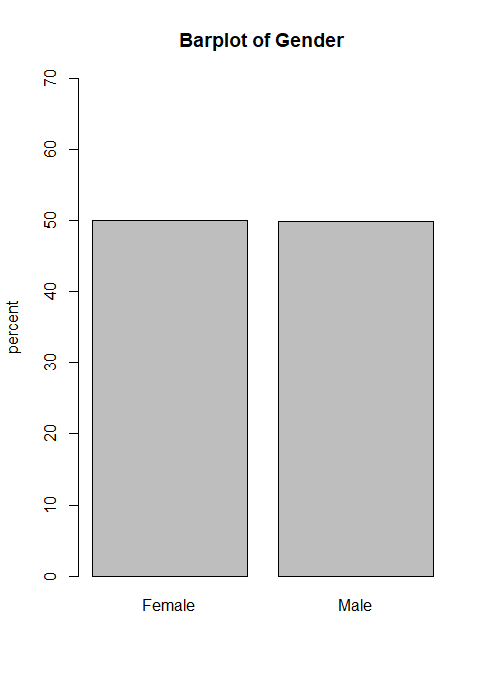
\includegraphics[width=0.5\linewidth]{screenshot006}
	\caption{Gender statistics barplot}
	\label{fig:genderbar}
\end{figure}
Figure \ref{fig:genderbar} shows a barplot of the gender. It shows that the males have a percentage of 49.9\%; a total of 499 and the females have a percentage of 50.1\%; a total of 501.
\section{The estimates of the fitted GLM models}
The parameters of the fitted  GLM model are estimated using the maximum likelihood estimation method. The fitting was done and summaries where total sales is the response variable.
A generalized linear model with Gamma distribution was fitted to the data and summary of estimates was obtained. 
\begin{table}[H]
\centering
\caption{Parameter estimates of the fitted Gamma model}	
	\begin{tabular}{ccccc}
		\hline
		Variable   & Parameter & se(parameter) & p-value & exp(parameter) \\ \hline
		Intercept  & 3.0425 & 0.0559     & 0.0000  & 20.9573        \\
		Unit price & 0.0209 & 0.0559     & 0.0000  & 1.0211         \\
		Quantity   & 0.2220 & 0.0070     & 0.0000  & 1.2485         \\
		Tax        & 0.0003 & 0.0023     & 0.8800  & 1.0003         \\
		Rating     & 0.0039 & 0.0051     & 0.4400  & 1.0039         \\
		Gender     & 0.0064 & 0.0175     & 0.7160  & 1.0064         \\ \hline
	\end{tabular}
\label{table:gamma}
\end{table}
 Table \ref{table:gamma} shows the estimated parameters of the total sales using GLM with Gamma model. The coefficient estimate in the output indicates the average change in the log odd of the response variable with a unit increase in each predictor variable for example, a unit increase in the predictor variable unit price is associated with an average change of 0.0208 in the log odds of the response variable. This means higher values of the unit price are associated with a higher likelihood of the response variable. The standard error  gives an idea of the  variability associated with coefficient estimate. This essentially tells us how well each predictor variable is able to predict the value of the response variable in the model. The variables unit price, quantity and tax are significant at 5\% level. The coefficients for unit price, quantity, rating, gender and tax estimates are positive indicating positive correlation with the response variable.
  
\begin{table}[H]
	\centering
	\caption{Parameter estimates of the fitted Inverse Gaussian model}
	\begin{tabular}{ccccc}
		\hline
		Variable   & Parameter  & se(parameter) & p-value & exp(parameter) \\ \hline
		Intercept  & 0.0215 & 0.0005     & 0.0000  & 1.0218         \\
		Unit price & -0.0002 & 0.0000     & 0.0000  & 0.9998         \\
		Quantity   & -0.0019 & 0.0001     & 0.0000  & 0.9981         \\
		Tax        & 0.0003 & 0.0000     & 0.0000  & 1.0003         \\
		Rating     & -0.0000 & 0.0000     & 0.4660  & 1.0000         \\
		Gender     & -0.0000 & 0.0001     & 0.7610  & 1.0000         \\ \hline
	\end{tabular}
\label{table:inverse}
\end{table}
Table \ref{table:inverse} shows the estimated parameters of the total sales using a GLM with Inverse Gaussian distribution. The p-value is used in checking the significant variables. The variables; unit price, quantity and tax are significant at 5\% level of significance. The significant variables shows there is correlation  with the response variable. The coefficients for unit price, quantity, rating and gender are negative implying negative correlation with the response variable while the coefficient for tax estimate is positive indicating positive correlation with the response variable. The standard error provides the absolute measure of the typical distance that the data points fall from the regression line. 

\begin{table}[H]
	\centering
	\caption{Parameter estimates of the fitted Gaussian model}
	\begin{tabular}{ccccc}
		\hline
		Variable   & Parameter & se(parameter) & p-value & exp(parameter) \\ \hline
		Intercept  & 0.0113    & 0.0004        & 0.0000  & 1.0113         \\
		Unit price & -0.0001   & 0.0000        & 0.0000  & 0.9999         \\
		Quantity   & -0.0008   & 0.0001        & 0.0000  & 0.9992         \\
		Tax        & 0.0001    & 0.0000        & 0.0000  & 1.0000         \\
		Rating     & 0.0000    & 0.0000        & 0.8320  & 1.0000         \\
		Gender     & 0.0000    & 0.0001        & 0.8960  & 1.0000         \\ \hline
	\end{tabular}
\label{table:Gaussian}
\end{table}
Table \ref{table:Gaussian} shows the estimated parameters of the total sales using GLM with Gaussian distribution. The coefficient estimate in the output indicates the average change in the response variable with a unit increase in each predictor variable for example, a unit increase in the predictor variable unit price is associated with an average change of -0.0001 in the response variable. This means that the higher values of the unit price are associated with lower values of the response.  The variables unit price, quantity and tax are significant at 5\% significance level. The coefficients for unit price and quantity are negative implying negative correlation with the response variable while the coefficient for tax estimate is positive indicating positive correlation with the response variable. The standard error  gives an idea of the  variability associated with coefficient estimate. For example the variability associated with unit price is 0.004.
\section{Model selection}
The AIC is a metric used to compare the fit of different regression models. The lower the value the better the regression model is able to fit the data. 
\begin{table}[H]
	\centering
	\caption{AIC values for selecting the model}
	\begin{tabular}{@{}cccc@{}}
		\toprule
		& Gamma & Inverse Gaussian & Gaussian \\ \midrule
		AIC & 8846  & 10183            & 9489     \\ \bottomrule
	\end{tabular}
\label{table:selection values}
\end{table}
Table \ref{table:selection values} shows the Akaike Information Criterion values for the three generalized linear models that is Gamma, Inverse Gaussian and Gaussian models. It can be seen that the model with inverse Gaussian has the highest value and the model with Gamma has the least AIC. This further implies that the Gamma model is considered to be a better fit for the data.
\section{Adequacy of the model}
To assess the adequacy of the fitted model, a Chi-square goodness of fit test at 5\% significance level was used. The model has a chi-square statistic 149019 and 799 degrees of freedom. The chi-square distribution returns a p-value of zero. Consequently the null hypothesis, in equation (\ref{eqn:chihypo}) is rejected at 5\% level of significance that the deviation between the observed and the expected is not significantly large and thus the model is a good fit to the data. 

\section{Prediction using the fitted model}
A GLM gamma model was chosen to forecast the sales. The gamma model took the equation of the form;
\begin{equation}
\centering
\label{eqn:forecasteqn}
	\hat{P}(Y|X) = \frac{exp((3.0420 + 0.0210 X_{1} + 0.2220 X_{2} + 0.0003 X_{3} + 0.0039 X_{4} + 0.0064 X_{5}))}{1+ exp(-(3.0420 + 0.0210 X_{1} + 0.2220 X_{2} + 0.0003 X_{3} + 0.0039 X_{4} + 0.0064 X_{5}))}
\end{equation}
where $g$ is the associated link function.
The Gamma GLM model was used to predict the sales and a sample of the predictions are given.
\begin{table}[H]
	\centering
	\caption{Actual and Predicted sales values}
	\begin{tabular}{lll}
		\hline
		No. & Actual  & Predicted \\ \hline
		801 & 144.963 & 133.514   \\
		802 & 253.680 & 238.089   \\
		803 & 495.317 & 421.726   \\
		804 & 462.672 & 446.291   \\
		805 & 714.326 & 781.299   \\
		806 & 325.374 & 262.224   \\
		807 & 195.678 & 236.977   \\
		808 & 210.966 & 151.038   \\ \hline
	\end{tabular}
\label{table:values}
\end{table}
Table \ref{table:values} shows the first eight values of the predicted and actual sales using GLM with Gamma model. The values show that the model generated values that reflect the actual values; implying that the forecasts were accurate. 
\begin{figure}[H]
	\centering
	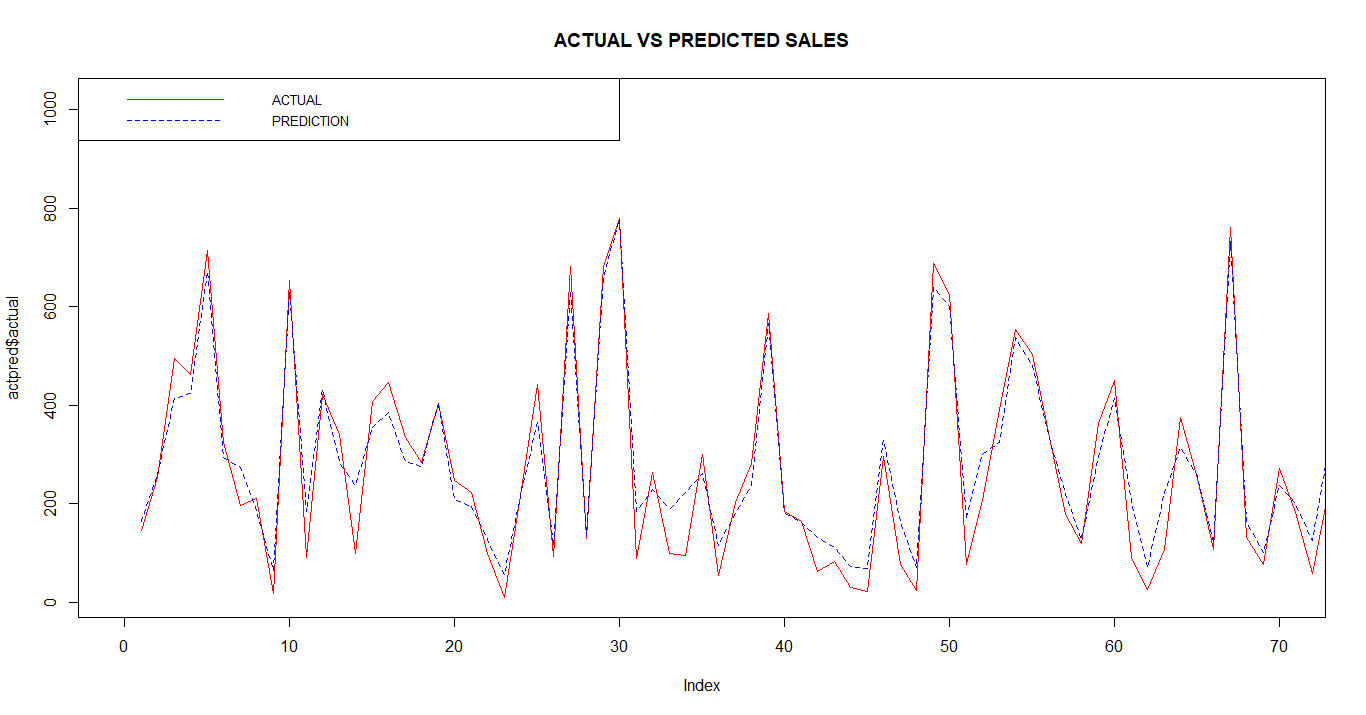
\includegraphics[width=0.9\linewidth]{screenshot005}
	\caption{Plot of Actual and predicted sales}
	\label{fig:plot accuracy}
\end{figure}

Figure \ref{fig:plot accuracy} shows the plot of the actual and forecasted sales. The plot shows that the sales forecast are not far from the actual observed sales. This shows that the GLM Gamma model fitted was a good choice for the sales data.
\section{The accuracy of the sales forecast}
 The accuracy of the sales forecast was checked using the mean square error formula in equation (\ref{eqn:MSE}).
 Mean square error measures the average of squares of errors. A large MSE indicates wide dispersion from the actual values while lower values indicates closeness to the actual values which further implies the prediction model is accurate. An MSE value of 0.0603 was obtained  which shows that the forecast were accurate.



